\documentclass[12pt,english]{article}
\usepackage[T1]{fontenc}
\usepackage[utf8]{inputenc}
\usepackage{tgpagella}
\usepackage{mathpazo}
\usepackage{microtype}
\usepackage[margin=2.5cm]{geometry}
\usepackage{setspace}
\onehalfspacing
\usepackage{babel}
\usepackage{csquotes}
\usepackage{booktabs}
\usepackage{makecell}
\usepackage{graphicx}
\usepackage{amsmath}
\usepackage{xcolor}
\usepackage{textcomp}
\usepackage{lineno}
\usepackage{bibunits}
\usepackage[round,authoryear,sort&compress]{natbib}
\defaultbibliographystyle{plainnaturl_clean}
\usepackage[colorlinks=true,linkcolor=blue!60!black,citecolor=blue!60!black,urlcolor=blue!60!black,backref=true]{hyperref}

% Limites de l'exercice : les répondants n'avaient pas le pour et contre des mesures. Prometteur : on pourrait demander à une convention citoyenne de plancher sur le sujet, ça permettrait de créer du consensus dans la population.
% Tout parti doit être sérieux sur le budget s'il veut gagner.
% Éliminer doublons: ptet pas 9 Mds (Ravignon dit 7.5), mais il faut ajouter d'autres mesures consensuelles de rationalisation des dépenses: baisse des prix des produits de santé 2.65,  Généralisation de la massification des achats et de la mutualisation des circuits entre les collectivités 3...
% gel du point d'indice pendant 5 ans: 20.7 https://www.cfdt-ufetam.org/pas-de-hausse-du-point-dindice-ni-de-prime-gipa-pour-les-agents-publics-en-2025/

\title{Préférences budgétaires des Français :\\
résultats d'une enquête représentative}
\author{Adrien Fabre\thanks{CNRS; CIRED. Données, code et figures disponibles sur
\url{https://github.com/bixiou/budget_26}.}}
\date{Avril 2026}

\begin{document}
\maketitle

% \linenumbers

\begin{abstract}
Quelles mesures les Français sont-ils prêts à accepter pour réduire le déficit public~? J'analyse les résultats d'une enquête menée en 2026 sur un échantillon représentatif de 1\,000 Français. Pour 30~mesures de consolidation budgétaire, les répondants indiquent si elle leur paraît souhaitable, convenable, supportable ou inacceptable. Les Français préfèrent les mesures de rationalisation de la dépense publique, les taxes sur les plus riches et la suppression des aides aux étrangers~; ils rejettent la hausse de l'âge de départ à la retraite et les hausses de taxes touchant tous les ménages (TVA, CSG). Par ailleurs, une majorité souhaite %réduire le déficit, 
améliorer les services publics, augmenter le SMIC, ou encore une plus grande fermeté judiciaire. La tripartition entre gauche, centre-droit/droite et extrême-droite émerge naturellement des préférences programmatiques. La gauche se distingue principalement sur la question des étrangers, le centre-droit/droite sur celle des retraites. Il sera difficile de constituer une majorité~: alors que la majorité souhaite stabiliser l'endettement public, au plus 34\% des Français accepteraient toutes les mesures d'un programme atteignant cet objectif. 
L'insatisfaction envers l'ensemble des partis politiques se matérialise par une dispersion des préférences individuelles, bien plus variées au sein des électeurs d'un même parti qu'entre préférences moyennes des électeurs de partis différents. 
\end{abstract}

\clearpage
\tableofcontents
\newpage

% TODO: weight
% TODO: open questions

%%%%%%%%%%%%%%%%%%%%%%%%%%%%%%%%%%%%%%%%%%%%%%%%%%%%%%%%%%%%%
\section{Introduction}
\label{sec:intro}
%%%%%%%%%%%%%%%%%%%%%%%%%%%%%%%%%%%%%%%%%%%%%%%%%%%%%%%%%%%%%

La France fait face à un déficit public structurel significatif. Selon le \citet{CAE2025}, ramener la dette publique sur une trajectoire soutenable nécessiterait un effort d'environ 112~milliards d'euros à l'horizon 2030, par une combinaison de hausses de recettes et de baisses de dépenses. 
% La question n'est pas seulement économique~: elle est profondément politique. 
Les Français sont-ils prêts à une telle consolidation budgétaire~? Quelles mesures sont-ils disposés à accepter~? Une majorité peut-elle se dégager sur un programme budgétaire~?

J'ai mené une enquête sur un échantillon représentatif de 1~000 Français pour répondre à ces questions. Je me suis inspiré de trois initiatives récentes sur le sujet. Le \cite{CAE2025} a publié une note et développé un \href{https://claude.ai/public/artifacts/74cd0701-a4f0-499e-a409-cae1da524ee4}{outil interactif} permettant à chacun de composer son propre programme de réduction du déficit. La \href{https://laplateformeprogressiste.org/wp-content/uploads/2025/12/20251210_Resultats-par-mesure-1.pdf}{Plateforme Progressiste} a organisé fin 2025 une conférence de consensus en ligne permettant à ses sympathisants de s'informer et de voter sur différentes propositions budgétaires\footnote{Cette plateforme a été cofondée par Pascal Canfin, Sarah Faivre et Éric Hazan, avec pour vocation d'élaborer un programme pour le centre-gauche. Les différentes mesures soumises au vote des sympathisants ont été sélectionnées et chiffrées par un collectif d'économistes incluant Jean Pisani-Ferry, Olivier Blanchard, Antoine Bergeaud, Anne Epaulard et Pascal Saint-Amans.}. Enfin, le citoyen Adrien Abécassis a créé le simulateur \href{budget-citoyen.fr}{budget-citoyen.fr}, proposant au grand public de choisir son budget préféré en faisant varier les postes de dépenses, de recettes, ou en sélectionnant des mesures pré-définies. Ces démarches partagent l'ambition d'identifier des mesures de réduction du déficit en vue du prochain quinquennat.

% Notre enquête adopte une approche complémentaire~: plutôt que de demander aux répondants de composer eux-mêmes un budget équilibré, nous leur soumettons une liste de mesures concrètes et mesurons le niveau d'acceptabilité de chacune. Cela permet d'analyser les déterminants du soutien, les distances entre groupes électoraux, les typologies de répondants et de mesures, et — surtout — d'identifier des \emph{paquets majoritaires}~: des ensembles de mesures pour lesquels une même majorité des citoyens soutient simultanément chacune des mesures du paquet.

La note est organisée comme suit. La section~\ref{sec:methode} détaille la méthode et la représentativité de l'échantillon. La section~\ref{sec:resultats} présente les résultats descriptifs. La section~\ref{sec:determinants} analyse les déterminants du soutien. La section~\ref{sec:paquets} identifie les paquets de mesures acceptables conjointement par une majorité d'électeurs. La section~\ref{sec:ecarts} examine les distances entre groupes électoraux. La section~\ref{sec:clusters} présente les typologies de répondants et de mesures. La section~\ref{sec:progressistes} compare les résultats à l'exercice des \textit{Progressistes}. La section~\ref{sec:conclusion} conclut. 


\section{Méthode}
\label{sec:methode}
%%%%%%%%%%%%%%%%%%%%%%%%%%%%%%%%%%%%%%%%%%%%%%%%%%%%%%%%%%%%%

\subsection{Questionnaire}

Après avoir renseigné leurs caractéristiques sociodémographiques et leur vote aux élections européennes de 2024, deux questions sont posées aux répondants~:

\begin{itemize}
  \item \textbf{Question \texttt{programme}}~: \textit{Pour chacune des mesures ci-dessous, sa présence dans le programme d'un candidat à l'élection présidentielle de 2027 vous rendrait-elle plus ou moins favorable à ce candidat~?} \\ Les répondants doivent choisir une valeur parmi 5 (de \textit{Beaucoup moins} à \textit{Beaucoup plus favorable}) pour 17 mesures, présentées dans un ordre aléatoire. 
  \item \textbf{Question \texttt{budget}}~:\textit{Le déficit public français s'est établi à 5~\% du PIB en 2025. \textbf{Le Conseil d'Analyse Économique recommande de} le ramener à 2,7~\% du PIB afin de stabiliser la dette et se prémunir contre une prochaine crise économique. Cela implique de \textbf{prendre des mesures d'économie pour un total de 90 milliards d'euros} dans les cinq prochaines années.\\

Voici une liste de mesures de réduction des dépenses ou de hausse des recettes, avec le montant que chacune permettrait d'économiser.
\textbf{Veuillez indiquer votre évaluation pour chaque mesure}~: \textit{souhaitable} quel que soit l'objectif de réduction du déficit, \textit{convenable} dans l'optique de réduction du déficit, \textit{supportable} dans cette optique, ou au contraire \textit{inacceptable}.\\
Le total des économies réalisées par les mesures \textit{convenables} ou \textit{souhaitables} est affiché à gauche.} \\ Les répondants doivent choisir une valeur parmi les quatre décrites ou \textit{Ne sais pas} pour 30 mesures, avec l'économie budgétaire qu'elles représentent entre parenthèses.
\end{itemize}

% L'enquête comprenait ensuite des questions sur d'autres sujets qui ne sont pas analysées dans cette note.

\subsection{Échantillon et pondération}

L'enquête a été conduite en ligne auprès de 1\,000~résidents français adultes entre les 6 et 20 mars 2026 via Bilendi. 
L'échantillon a été pondéré par raking (calage) sur le genre, l'âge, le revenu, le niveau de diplôme, l'urbanité et la région, de façon à correspondre aux distributions de la population française.

Le tableau~\ref{tab:representativite} présente les statistiques de représentativité. L'échantillon brut présente une légère sur-représentation des revenus faibles (Q1~: 31\,\% vs 25\,\%) et des diplômés du supérieur (33\,\% vs 26\,\%) ainsi qu'une sous-représentation des abstentionnistes (31\,\% vs. 51\,\%). La pondération corrige ces déséquilibres sauf pour le vote, exclu de la pondération car les gens ont tendance à sous-déclarer leur abstentionnisme \citep{sciarini_turnout_2016}.

\begin{table}[htbp]
  \centering
  \caption{Représentativité de l'échantillon}
  \label{tab:representativite}
  
\begin{tabular}[t]{lcc}
\toprule
% \multicolumn{1}{c}{} & \multicolumn{2}{c}{France} \\
% \cmidrule(l{3pt}r{3pt}){2-3}
  & Pop. & Échantillon\\
\midrule
% Taille de l'échantillon &  & 1~000\\
% \addlinespace
Genre: Femme & .52 & .52\\
Genre: Homme & .48 & .48\\
\addlinespace
Niveau de vie: quartile Q1 ($<$ 18k\texteuro{}) & .25 & \textbf{.31}\\
Niveau de vie: quartile Q2 (18--25k\texteuro{})  & .25 & .22\\
Niveau de vie: quartile Q3 (25--34k\texteuro{}) & .25 & .23\\
Niveau de vie: quartile Q4 ($>$ 34k\texteuro{})  & .25 & .24\\
\addlinespace
Âge: 18--24 & .10 & .11\\
Âge: 25--34 & .15 & .13\\
Âge: 35--49 & .23 & .22\\
Âge: 50--64 & .24 & .27\\
Âge: 65+ & .27 & .28\\
\addlinespace
Diplôme 25--64: Brevet ou aucun & .10 & .09\\
Diplôme 25--64: Baccalauréat, CAP ou BEP & .26 & \textbf{.20}\\
Diplôme 25--64: Bac +2 ou plus & .26 & \textbf{.33}\\
\addlinespace
Urbanité: Grand pôle urbain & .47 & .50\\
Urbanité: Couronne d'un grand pôle & .19 & .17\\
Urbanité: Autre (rural) & .34 & .32\\
\addlinespace
Région: Île-de-France & .18 & .21\\
Région: Nord \& Est & .22 & \textbf{.15}\\
Région: Sud-Ouest & .11 & \textbf{.13}\\
Région: Sud-Est & .21 & .23\\
Région: Ouest & .28 & .27\\
\addlinespace
Vote européennes: Gauche & .17 & \textbf{.23}\\
\textit{Vote ou affinité: La France insoumise} & \textit{.082} & \textit{.075} \\ % .099
\textit{Vote ou affinité: Parti Communiste Français} & \textit{.020} & \textit{\textbf{.014}} \\ % .024
\textit{Vote ou affinité: Les Écologistes -- EÉLV} & \textit{.045} & \textit{\textbf{.062}} \\ % .055
\textit{Vote ou affinité: Parti Socialiste \& Place publique} & \textit{.114} & \textit{.113} \\ % .138
\textit{Vote ou affinité: Parti animaliste} & \textit{.017} & \textit{\textbf{.011}} \\ % .02
Vote européennes: Centre-droit ou Droite & .12 & \textbf{.22}\\
\textit{Vote ou affinité: Renaissance, MoDem \& Horizons} & \textit{.121} & \textit{.134} \\ % .146
\textit{Vote ou affinité: Les Républicains} & \textit{.060} & \textit{\textbf{.110}} \\ % .073
\textit{Vote ou affinité: Résistons (Jean Lassalle)} & \textit{.019} & \textit{\textbf{.007}} \\ % .023
Vote européennes: Extrême-droite & .19 & \textbf{.24}\\
\textit{Vote ou affinité: Rassemblement National} & \textit{.259} & \textit{.276} \\ % .314
\textit{Vote ou affinité: Reconquête} & \textit{.045} & \textit{\textbf{.025}} \\ % .055
Vote européennes: Abstention, non-réponse ou Autre & .51 & \textbf{.31}\\
\bottomrule
\end{tabular}
  \par\smallskip
  {\footnotesize Note~: Les valeurs en gras indiquent un écart supérieur à 20\% entre l'échantillon et la population. La pondération ramène les proportions proches de celles de la population.}
\end{table}


%%%%%%%%%%%%%%%%%%%%%%%%%%%%%%%%%%%%%%%%%%%%%%%%%%%%%%%%%%%%%
\section{Résultats descriptifs}
\label{sec:resultats}
%%%%%%%%%%%%%%%%%%%%%%%%%%%%%%%%%%%%%%%%%%%%%%%%%%%%%%%%%%%%%

\subsection{Question \texttt{programme}}

La figure~\ref{fig:effect_program} présente le score moyen d'impact sur l'évaluation d'un candidat présidentiel pour chaque mesure.

\begin{figure}[htbp]
  \centering
  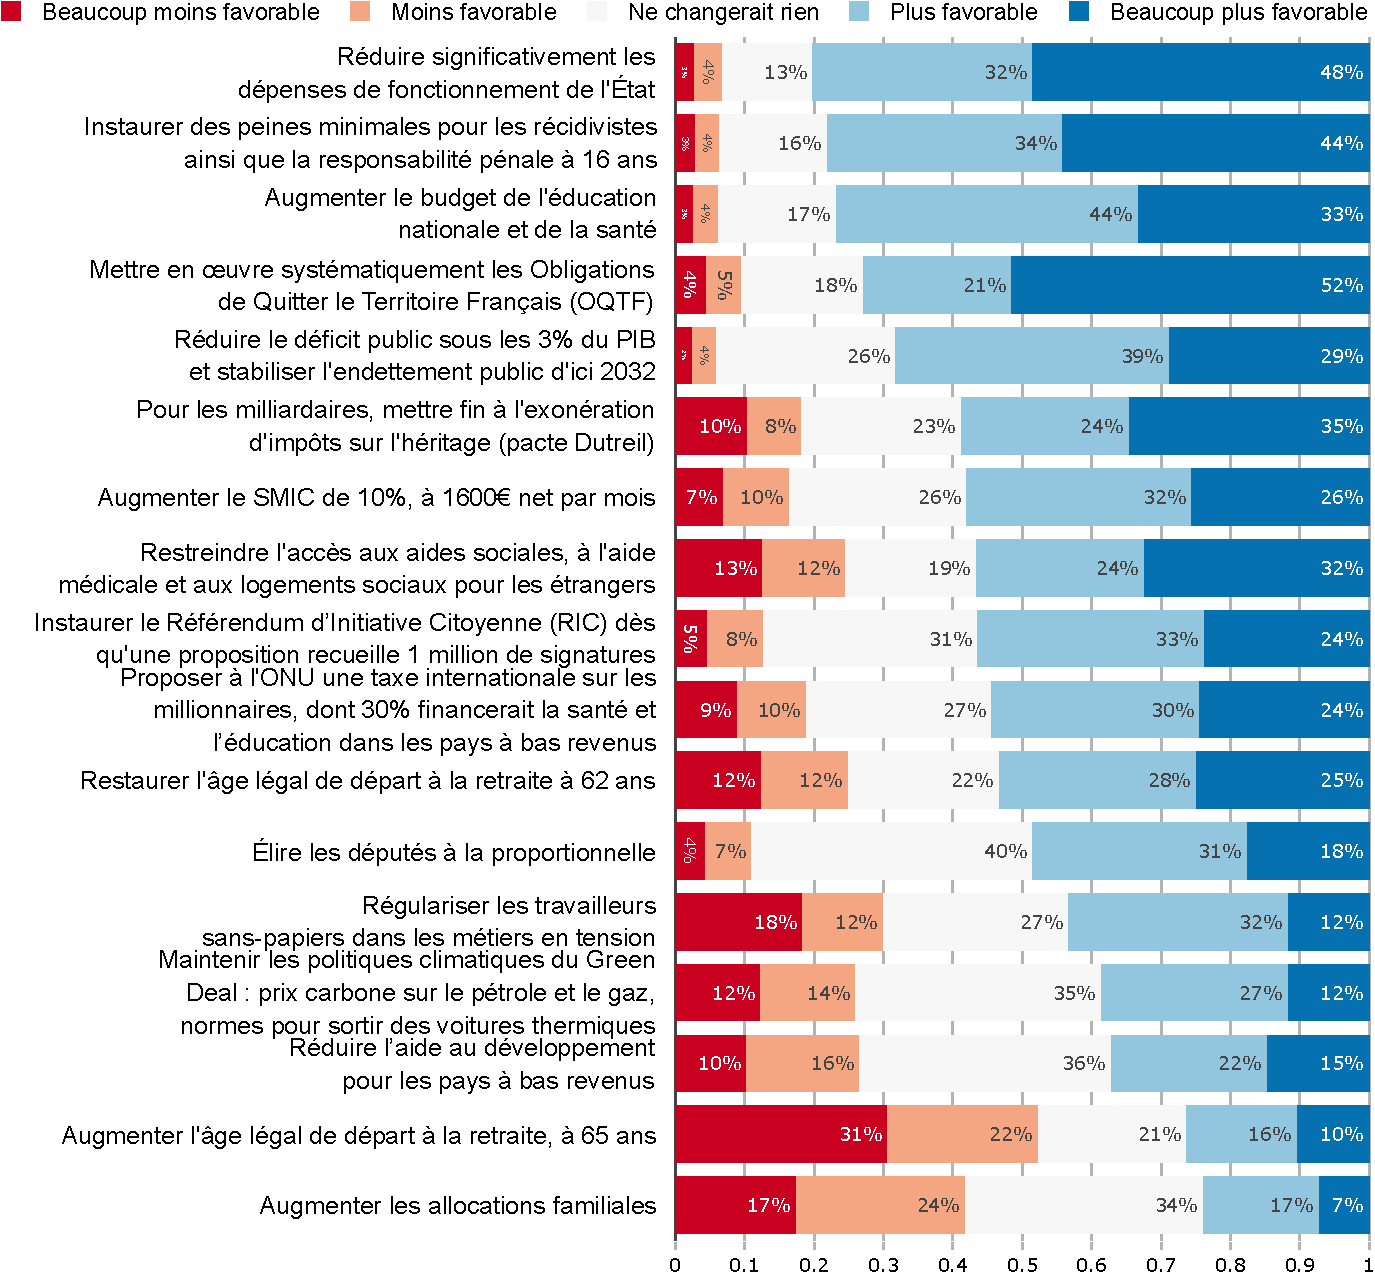
\includegraphics[width=\linewidth]{../figures/effect_program.pdf}
  \caption{Effet des mesures sur l'évaluation d'un candidat présidentiel (score moyen, échelle $-2$ à $+2$)}
  \label{fig:effect_program}
\end{figure}

Les mesures les plus valorisantes pour un candidat sont la réduction des dépenses de fonctionnement de l'État (+1,19), l'instauration de peines planchers (+1,12), l'application systématique des OQTF (+1,11) et l'augmentation du budget éducation et santé (+1,01). Cette dernière mesure est la seule à obtenir un score positif élevé dans \emph{tous} les groupes électoraux (non-votants~: +0,97~; centre-droit~: +0,90~; extrême droite~: +0,97~; gauche~: +1,22). Les Français souhaitent donc à la fois réduire le déficit, améliorer les services publics, augmenter le SMIC et une plus grande fermeté judiciaire.

La seule mesure à score négatif est le report de la retraite à 65~ans ($-0,50$), plébiscité uniquement par les électeurs de centre-droite (+0,46). Le retour du déficit sous les 3\,\% est modérément valorisant (+0,87).

L'application des OQTF et les peines planchers sont fortement clivantes~: très populaires à l'extrême droite (respectivement +1,83 et +1,67), elles sont nettement moins valorisées à gauche (+0,44 et +0,56).
\subsection{Question \texttt{budget}}

La figure~\ref{fig:budget} présente le soutien aux mesures budgétaires, classées par la proportion d'évaluations \textit{Convenable} ou \textit{Souhaitable}, hors \textit{Ne sais pas}. L'ensemble des réponses convenables pour une majorité totalise 31,5~milliards d'euros d'économies. Les économies atteignent 97,9~Mds en y ajoutant les mesures \textit{supportables} pour une majorité, et 24,8~Mds en se limitant aux mesures \textit{souhaitables} pour une majorité.

\begin{figure}[htbp]
  \centering
  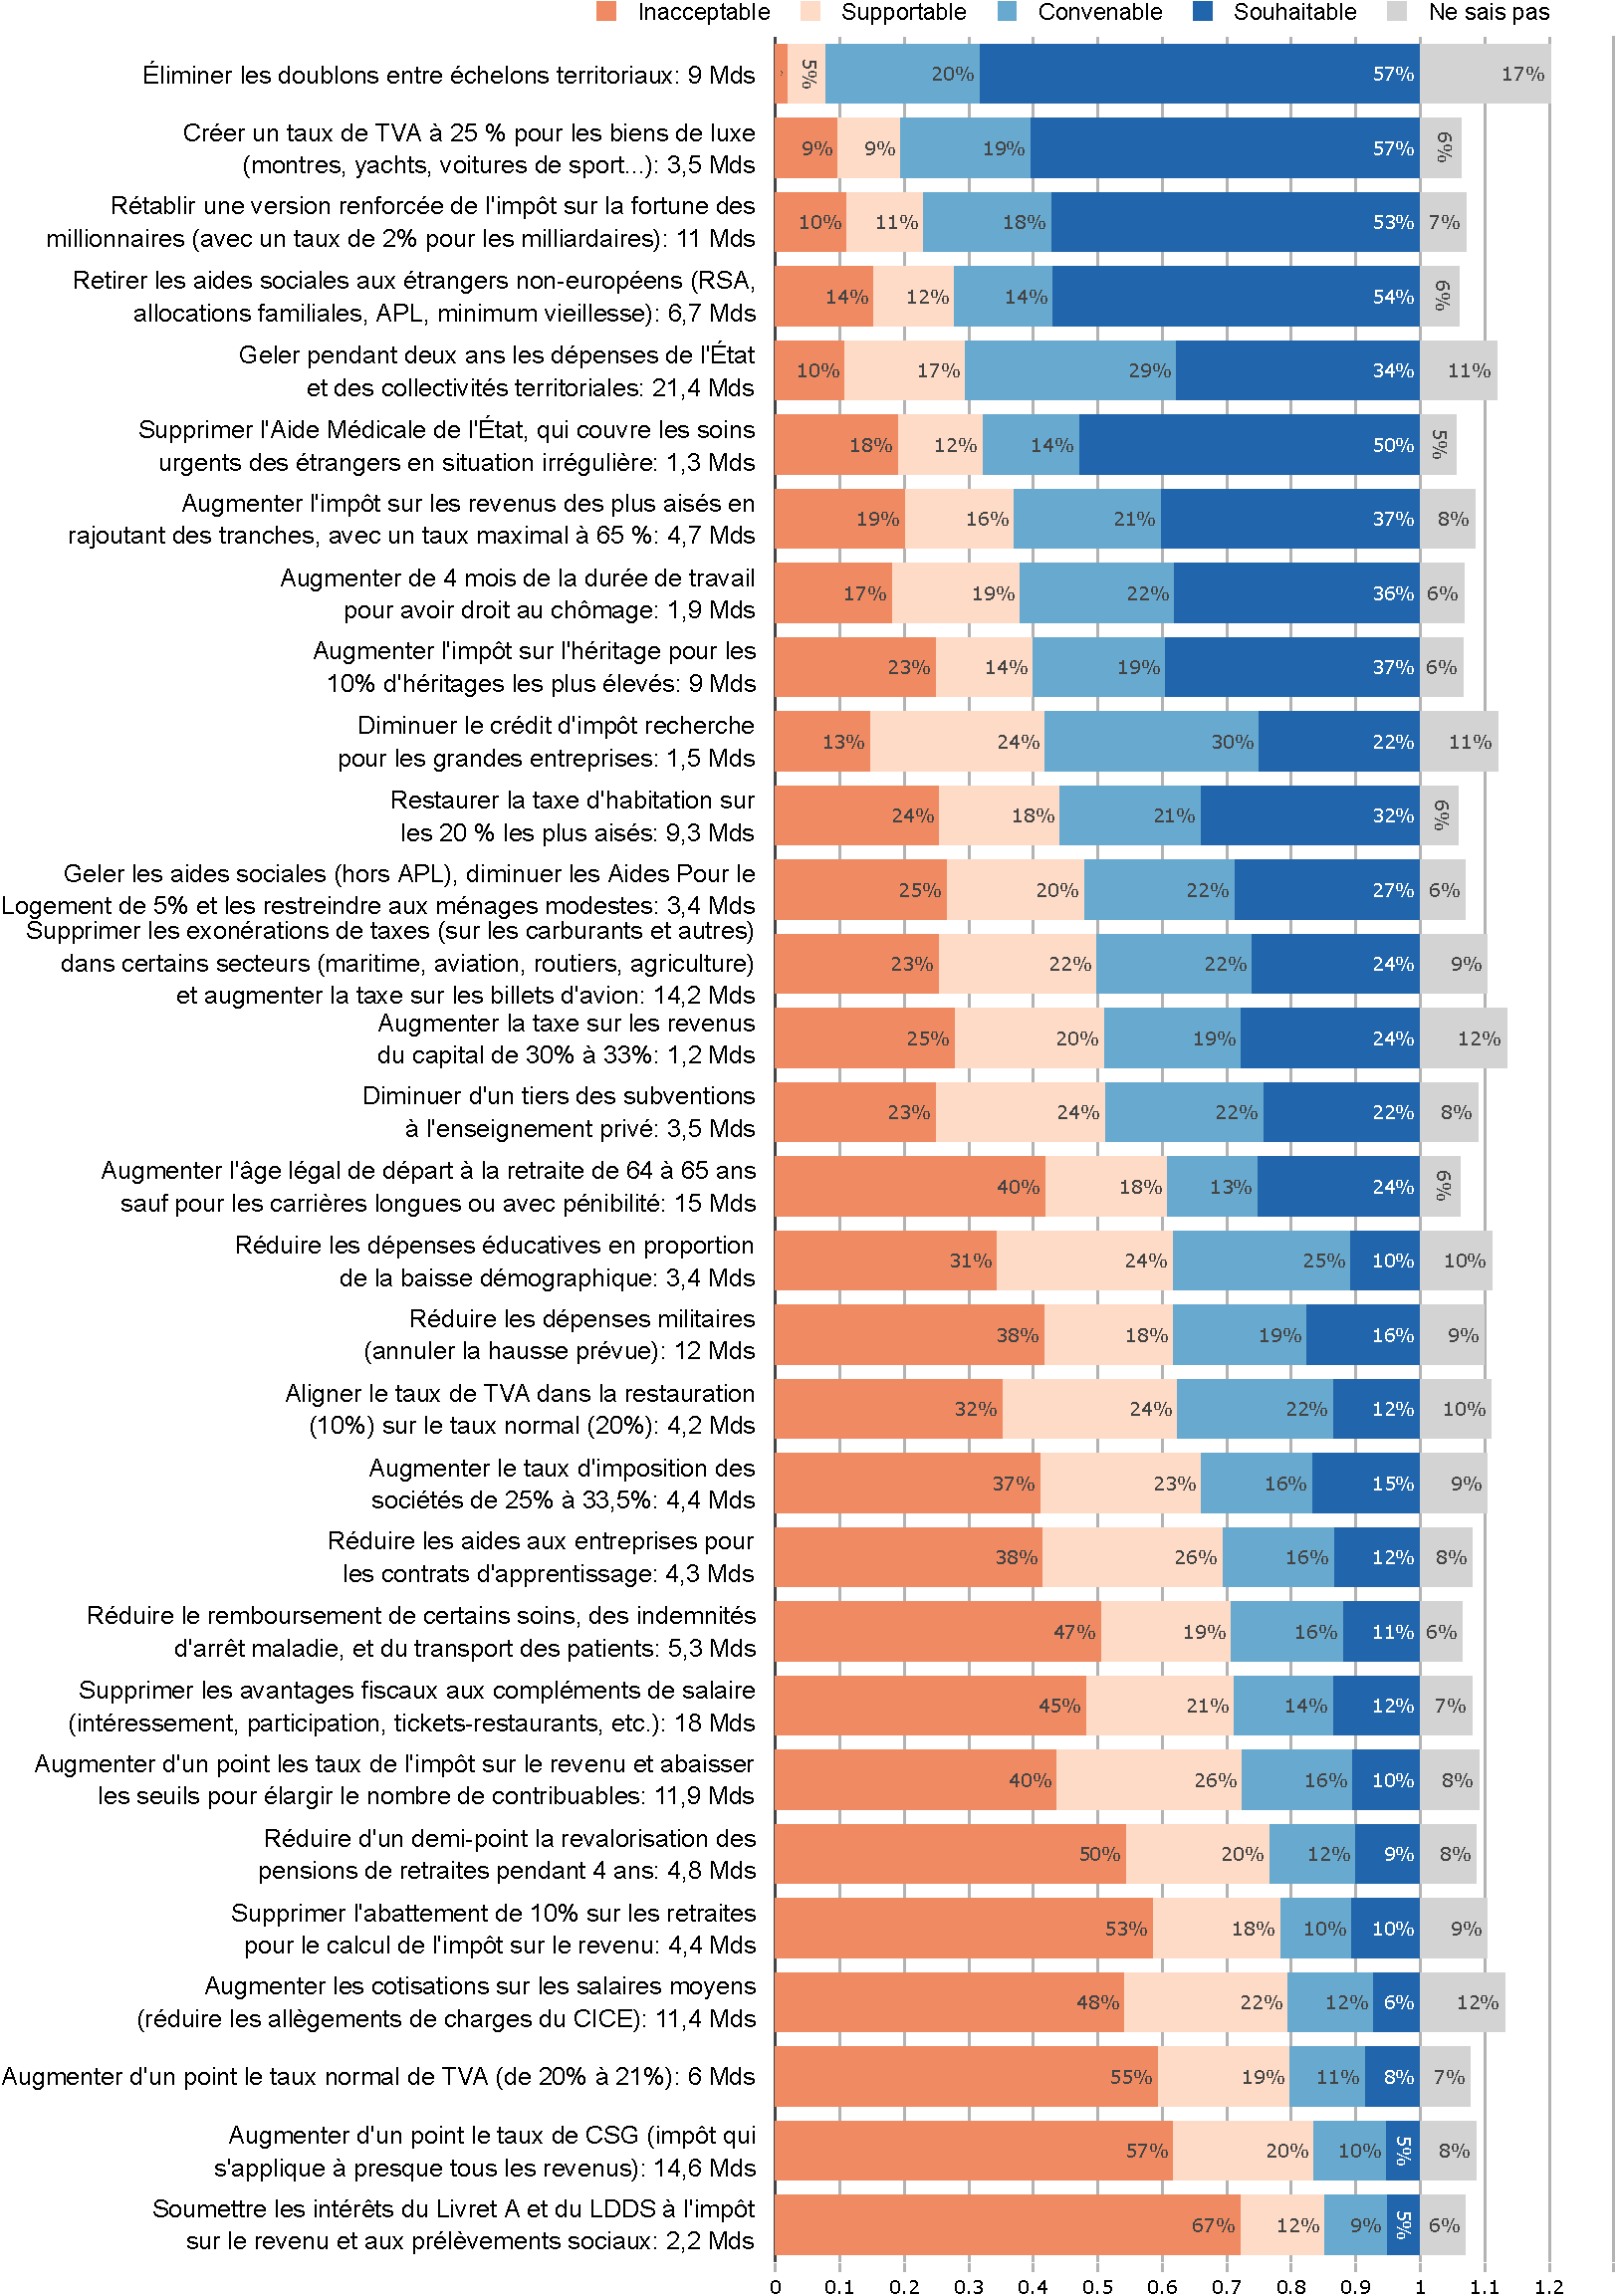
\includegraphics[width=\linewidth]{../figures/budget.pdf}
  \caption{Évaluations des mesures budgétaires.}
  \label{fig:budget}
\end{figure}

Cinq mesures recueillent plus de 50\,\% de réponses favorables (souhaitable ou convenable, incluant les NSP au dénominateur)~: l'élimination des doublons entre niveaux territoriaux (76,6\,\%, économie estimée~: 9~Mds€), la TVA à taux élevé sur les biens de luxe (74,5\,\%, 3,5~Mds€), le rétablissement de l'ISF (70,4\,\%, 11~Mds€), le retrait des aides sociales aux étrangers non-UE (69,5\,\%, 6,7~Mds€) et la suppression de l'AME (65,8\,\%, 1,3~Mds€). Le gel des dépenses de fonctionnement de l'État atteint 63,0\,\% (21,4~Mds€).

En excluant les NSP du dénominateur (taux \emph{xPNR}), les soutiens sont plus élevés~: élimination des doublons~92\,\%, TVA luxe~81\,\%, ISF~77\,\%, retrait des aides étrangers~72\,\%, suppression AME~68\,\%.

À l'inverse, les mesures les plus rejetées sont le report de l'âge de départ à la retraite à 65~ans (rejeté par une large majorité sauf chez les électeurs de centre-droite), les hausses de TVA et de CSG d'un point (rejetées par environ 80\,\% des répondants).

% \textbf{Lien avec le rendement budgétaire.} La corrélation entre le niveau de soutien à une mesure et son rendement budgétaire est faible~: certaines mesures très populaires (élimination des doublons, ISF) ont un rendement modéré, tandis que d'autres mesures potentiellement importantes (réforme des retraites, hausse de la CSG) sont impopulaires.


%%%%%%%%%%%%%%%%%%%%%%%%%%%%%%%%%%%%%%%%%%%%%%%%%%%%%%%%%%%%%
\section{Déterminants du soutien}
\label{sec:determinants}
%%%%%%%%%%%%%%%%%%%%%%%%%%%%%%%%%%%%%%%%%%%%%%%%%%%%%%%%%%%%%

Nous estimons pour chaque mesure \texttt{budget} une régression OLS du soutien (variable binaire : convenable ou souhaitable~= 1) en fonction du vote déclaré, du revenu, de l'âge, du genre et du niveau de diplôme (estimations pondérées). Les figures~\ref{fig:notes_groupes_budget} et~\ref{fig:notes_groupes_effect_program} présentent le niveau de soutien moyen par groupe électoral pour les deux questions.

\begin{figure}[htbp]
  \centering
  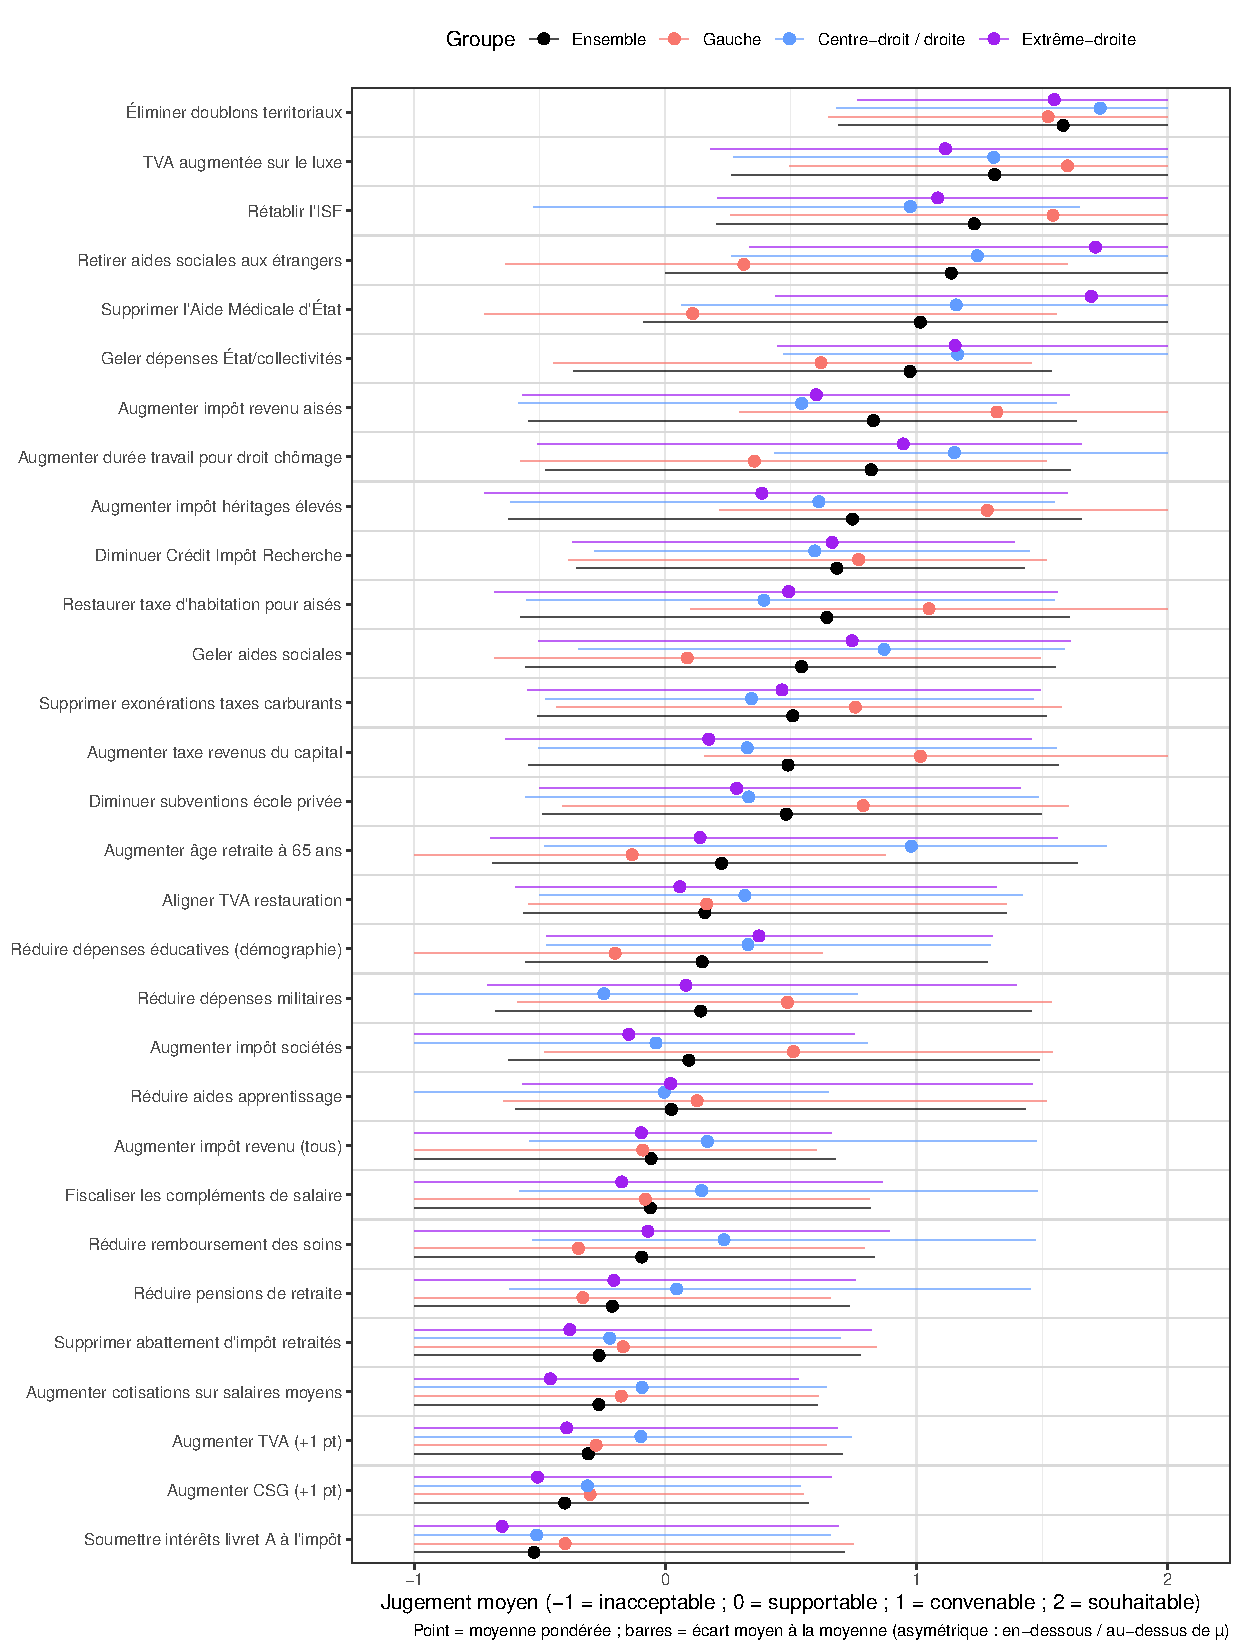
\includegraphics[width=\linewidth]{../figures/notes_groupes_budget.pdf}
  \caption{Soutien moyen aux mesures budgétaires par groupe électoral}
  \label{fig:notes_groupes_budget}
\end{figure}

\begin{figure}[htbp]
  \centering
  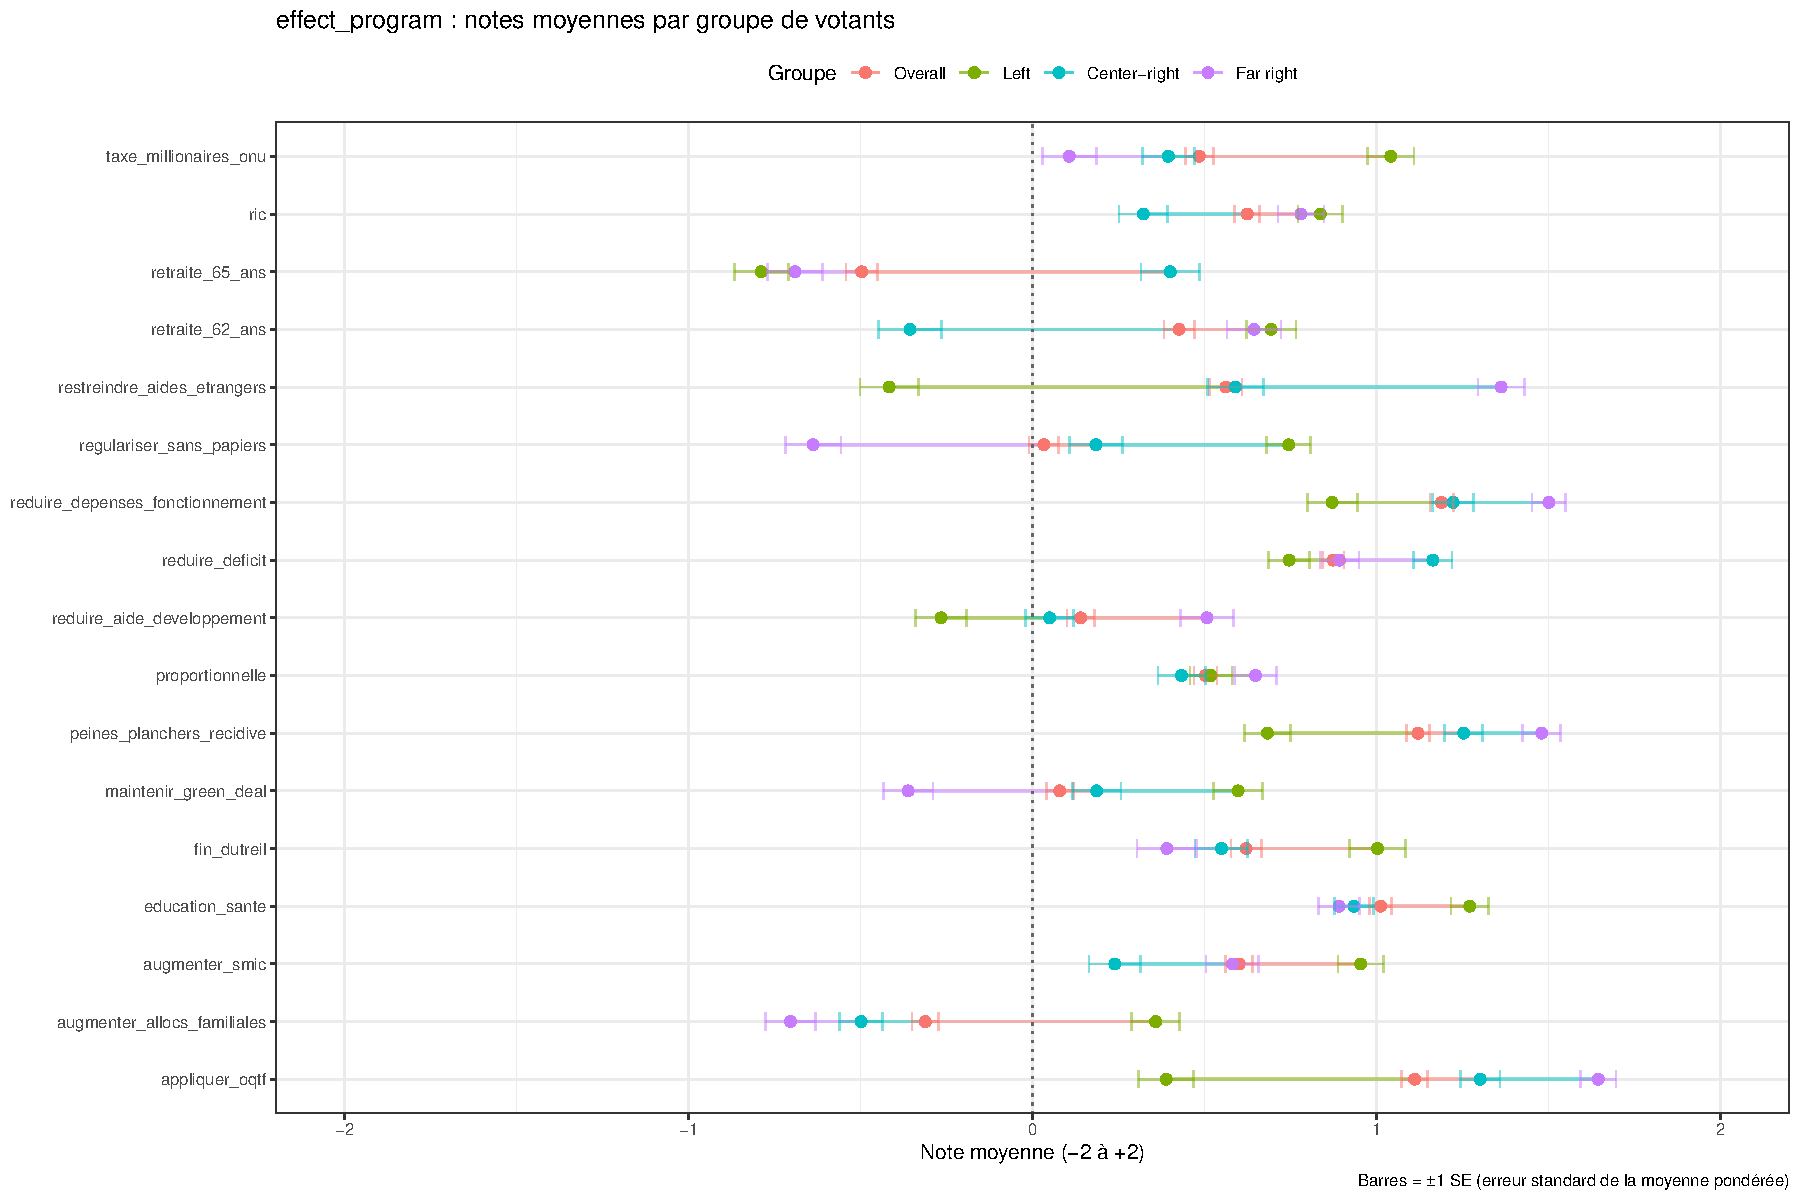
\includegraphics[width=\linewidth]{../figures/notes_groupes_effect_program.pdf}
  \caption{Score moyen d'impact électoral des mesures par groupe électoral}
  \label{fig:notes_groupes_effect_program}
\end{figure}

Les variables sociodémographiques (revenu, âge, genre, diplôme) n'expliquent collectivement qu'environ 5\,\% de la variance du soutien aux mesures. Le vote déclaré en explique également 5\,\%. Ensemble, ces deux blocs de variables en expliquent environ 9\,\% de la variance, soit nettement moins que les préférences idiosyncrasiques non capturées par ces caractéristiques.

\textbf{Vote.} C'est le déterminant le plus fort. Les électeurs de gauche soutiennent davantage les hausses d'impôts sur le patrimoine et s'opposent fortement aux mesures anti-immigration ($-36$~pp sur la suppression de l'AME, $-57$~pp sur le retrait des aides aux étrangers). Les électeurs de centre-droite soutiennent davantage le report de la retraite à 65~ans (+34~pp) et moins la réduction des dépenses militaires ($-16$~pp). Les électeurs de gauche s'opposent aussi davantage au gel des dépenses ($-15$~pp).

\textbf{Ce qui distingue la gauche.} Le clivage le plus net entre gauche et reste de l'électorat porte sur les mesures anti-immigration (retrait des aides aux étrangers, suppression de l'AME). Dans une moindre mesure, la gauche soutient davantage les taxes sur les riches (ISF, droits de succession, impôt sur les hauts revenus).

\textbf{Ce qui distingue le centre.} Les électeurs de centre-droite se distinguent principalement par leur soutien au report de l'âge de la retraite à 65~ans, et dans une moindre mesure par leur opposition aux hausses fiscales sur le patrimoine.

\textbf{Ce qui distingue l'extrême droite.} Les électeurs d'extrême droite partagent avec la gauche une forte opposition aux mesures de réduction de l'État providence (gel des aides sociales, coupes dans l'éducation) mais se rejoignent avec le centre sur les mesures anti-immigration.

\textbf{Âge.} Les jeunes (18--24 ans) soutiennent moins l'élimination des doublons ($-17$~pp), la suppression de l'AME ($-16$~pp) et le gel des dépenses ($-17$~pp).

\textbf{Revenu.} Le revenu est en grande partie non significatif, ce qui suggère que le clivage principal n'est pas économique mais culturel (le vote servant de proxy d'orientation idéologique).

%%%%%%%%%%%%%%%%%%%%%%%%%%%%%%%%%%%%%%%%%%%%%%%%%%%%%%%%%%%%%
\section{Paquets de mesures à majorité conjointe}
\label{sec:paquets}
%%%%%%%%%%%%%%%%%%%%%%%%%%%%%%%%%%%%%%%%%%%%%%%%%%%%%%%%%%%%%

Nous cherchons des ensembles de mesures tels qu'une même majorité de citoyens soutient simultanément chacune des mesures de l'ensemble. Formellement, un paquet $S$ est \emph{faisable} si la proportion pondérée de répondants qui soutiennent \emph{chaque} mesure de $S$ dépasse 50\,\% (avec les NSP exclus du dénominateur — convention \emph{xPNR}). Nous examinons deux définitions du soutien à une mesure.

\textbf{Algorithme.} Nous utilisons l'algorithme Apriori niveau par niveau~: en exploitant la propriété d'anti-monotonicité (tout sur-ensemble d'un paquet infaisable est infaisable), les candidats de taille $k$ sont générés uniquement à partir des paquets faisables de taille $k-1$, ce qui évite d'évaluer les sur-ensembles de paquets déjà infaisables.

La figure~\ref{fig:coalition_support_heatmap} présente le taux de soutien (conv+souh) à chaque mesure au sein de chaque coalition électorale. Elle révèle d'importantes disparités~: certaines mesures (élimination des doublons, TVA luxe) recueillent un soutien élevé dans tous les groupes, tandis que d'autres (retrait des aides aux étrangers, report de la retraite) sont fortement clivantes.

\begin{figure}[htbp]
  \centering
  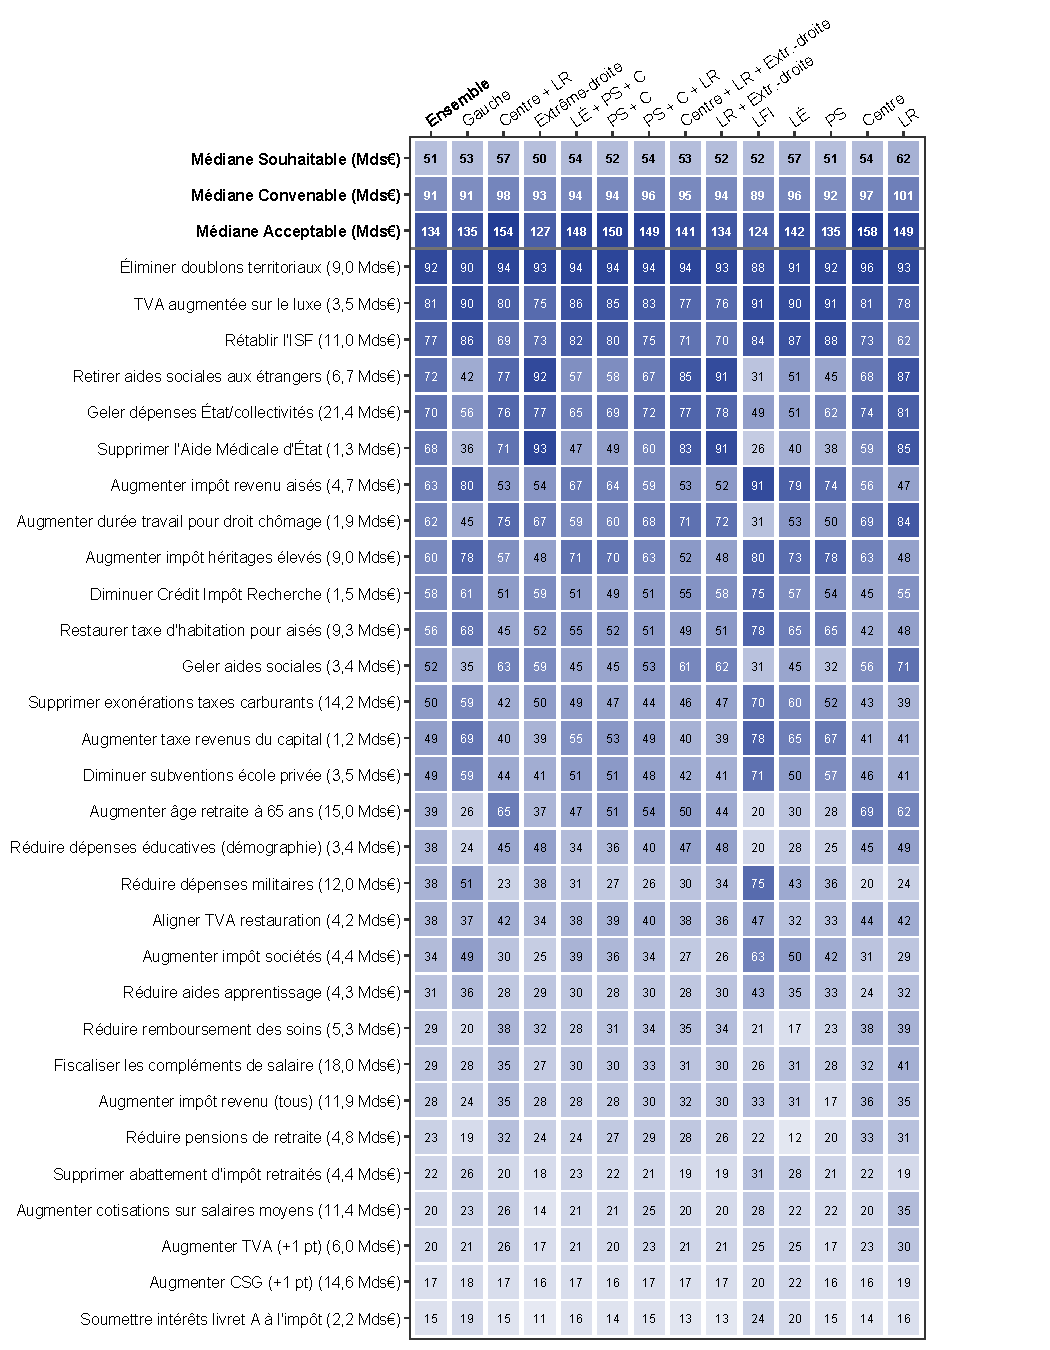
\includegraphics[width=\linewidth]{../figures/coalition_support_heatmap.pdf}
  \caption{Taux de soutien (conv+souh) par mesure et par coalition électorale}
  \label{fig:coalition_support_heatmap}
\end{figure}

La figure~\ref{fig:coalition_packages_matrix} présente les paquets de mesures à majorité conjointe identifiés pour chaque coalition. Quelle que soit la coalition envisagée, il n'existe pas de programme atteignant les 90~milliards d'euros nécessaires qui soit soutenu conjointement par une majorité~: une majorité d'électeurs trouvera toujours au moins une des mesures d'un tel paquet inacceptable. La coalition LÉ--LR (analogue au modèle SPD--CDU en Allemagne) converge vers des choix proches de l'ensemble de l'électorat, en épargnant davantage les mesures anti-immigration et les mesures fiscales sur les riches comparativement aux coalitions incluant le RN ou la LFI.

\begin{figure}[htbp]
  \centering
  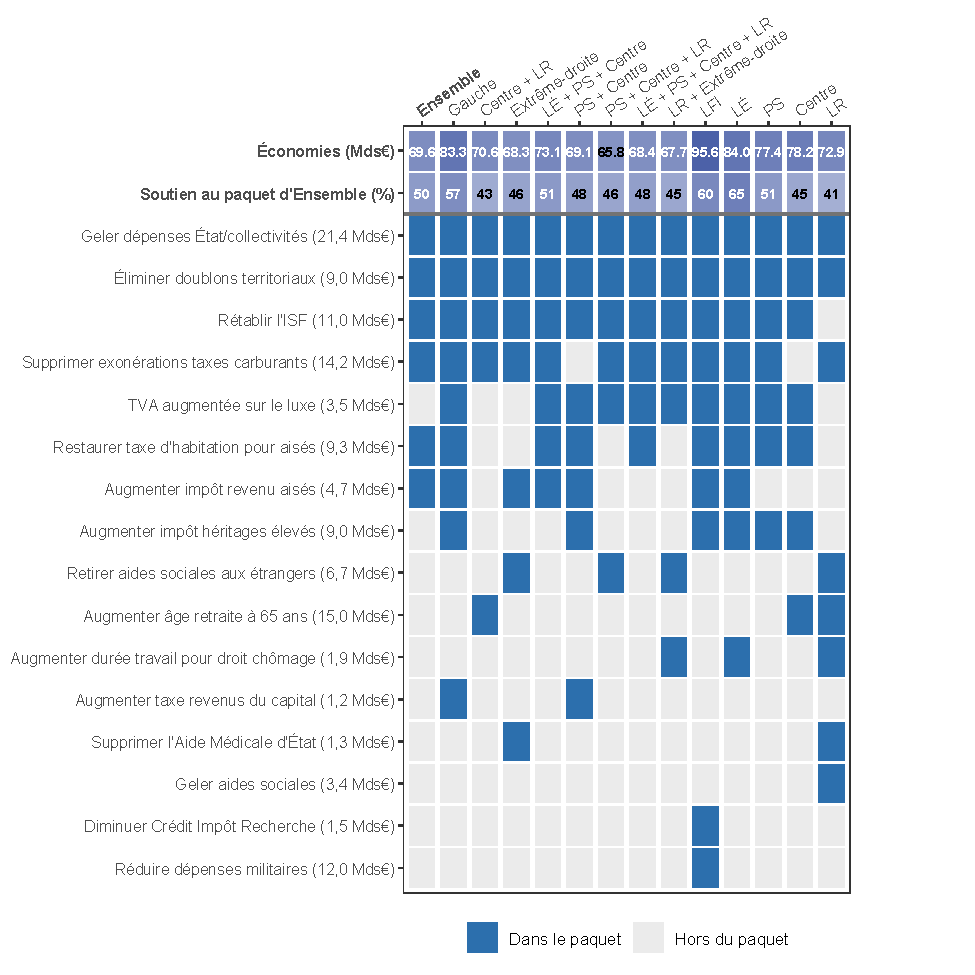
\includegraphics[width=\linewidth]{../figures/coalition_packages_matrix.pdf}
  \caption{Paquets de mesures à majorité conjointe par coalition électorale}
  \label{fig:coalition_packages_matrix}
\end{figure}

\subsubsection*{Définition stricte : convenable ou souhaitable (xPNR)}

Avec cette définition, 12~mesures ont un soutien individuel supérieur à 50\,\%. La recherche exhaustive sur leurs $2^{12} = 4\,096$ sous-ensembles montre qu'aucun paquet de 4~mesures ou plus n'atteint 50\,\% de soutien conjoint. Nous trouvons six paquets optimaux de 3~mesures (tableau~\ref{tab:paquets_strict}).

\begin{table}[htbp]
  \centering
  \caption{Paquets de 3 mesures à majorité conjointe — définition stricte (conv+souh, xPNR)}
  \label{tab:paquets_strict}
  \begin{tabular}{lcc}
    \toprule
    Mesures & Soutien conjoint & Économies (Mds€) \\
    \midrule
    Doublons + aides étrangers + AME & 58,8\,\% & 17,0 \\
    Doublons + ISF + TVA luxe & 57,9\,\% & 23,5 \\
    Doublons + aides étrangers + TVA luxe & 51,0\,\% & 19,2 \\
    Doublons + gel dépenses + aides étrangers & 51,7\,\% & 37,1 \\
    Gel dépenses + aides étrangers + AME & 50,6\,\% & 29,4 \\
    Aides étrangers + AME + TVA luxe & 50,1\,\% & 11,5 \\
    \bottomrule
  \end{tabular}
\end{table}

Le paquet au soutien conjoint le plus élevé (doublons + aides aux étrangers + AME, 58,8\,\%) est porté par une majorité très à droite~: extrême droite 34,9\,\% (vs 23,9\,\% dans l'ensemble), gauche 12,7\,\% (vs 23,0\,\%). Le paquet (doublons + ISF + TVA luxe, 57,9\,\%) a au contraire un profil plutôt gauche/centre. Ces deux majorités sont largement non superposables.

\subsubsection*{Définition élargie : supportable, convenable ou souhaitable (xPNR)}

En incluant les réponses « supportable » comme soutien, 23~mesures passent le seuil de 50\,\%. L'algorithme Apriori n'évalue que 2\,912~sous-ensembles (sur les $2^{23} = 8\,388\,608$ possibles). La taille maximale d'un paquet faisable passe à 6~mesures~; 15~paquets de cette taille dépassent 50\,\% de soutien conjoint (tableau~\ref{tab:paquets_large}).

\begin{table}[htbp]
  \centering
  \caption{Paquets de 6 mesures à majorité conjointe — définition élargie (supp+conv+souh, xPNR)}
  \label{tab:paquets_large}
  \small
  \begin{tabular}{lcc}
    \toprule
    Mesures & Soutien conjoint & Économies (Mds€) \\
    \midrule
    Doublons + gel dép. + aides étr. + AME + ISF + TVA luxe & \textbf{54,8\,\%} & 52,9 \\
    Doublons + gel dép. + aides étr. + AME + durée trav. + ISF & 52,6\,\% & 51,3 \\
    Doublons + gel dép. + aides étr. + AME + durée trav. + TVA luxe & 53,8\,\% & 43,8 \\
    Doublons + gel dép. + aides étr. + durée trav. + ISF + TVA luxe & 52,8\,\% & 53,5 \\
    Doublons + gel dép. + aides étr. + ISF + TVA luxe + IR aisés & 50,4\,\% & 56,3 \\
    Doublons + gel dép. + aides étr. + AME + durée trav. + gel aides & 51,9\,\% & 43,7 \\
    Doublons + gel dép. + AME + durée trav. + ISF + TVA luxe & 50,7\,\% & 48,1 \\
    Doublons + gel dép. + CIR + aides étr. + AME + durée trav. & 51,1\,\% & 41,8 \\
    Doublons + gel dép. + CIR + aides étr. + AME + ISF & 50,7\,\% & 50,9 \\
    Doublons + gel dép. + CIR + aides étr. + AME + TVA luxe & 50,1\,\% & 43,4 \\
    Doublons + gel dép. + CIR + aides étr. + ISF + TVA luxe & 50,0\,\% & 53,1 \\
    Doublons + CIR + aides étr. + AME + ISF + TVA luxe & 50,8\,\% & 33,0 \\
    Doublons + aides étr. + AME + durée trav. + ISF + TVA luxe & 53,3\,\% & 33,4 \\
    Doublons + aides étr. + AME + ISF + TVA luxe + IR aisés & 51,8\,\% & 36,2 \\
    Gel dép. + aides étr. + AME + durée trav. + ISF + TVA luxe & 51,8\,\% & 68,0 \\
    \bottomrule
  \end{tabular}
  \par\smallskip
  {\footnotesize Abréviations~: gel dép. = gel des dépenses État/collectivités~; aides étr. = retrait des aides aux étrangers non-UE~; durée trav. = allongement durée du travail/chômage~; gel aides = gel des aides sociales~; CIR = réduction du crédit impôt recherche~; IR aisés = hausse IR sur les ménages aisés.}
\end{table}

Le paquet au plus grand rendement (gel des dépenses + aides étrangers + AME + durée du travail + ISF + TVA luxe, 51,8\,\%, 68~Mds€) inclut à la fois des mesures anti-immigration et des mesures fiscales de gauche, ce qui correspond au profil « nationaliste » identifié en section~\ref{sec:clusters}. Le paquet au soutien conjoint le plus élevé (doublons + gel des dépenses + aides étrangers + AME + ISF + TVA luxe, 54,8\,\%, 52,9~Mds€) est modérément droitier~: extrême droite 28,4\,\% (+4,5~pp vs ensemble), centre-droite 26,3\,\% (+4,2~pp), gauche 17,9\,\% ($-5,1$~pp). Ce profil est nettement plus transpartisan que celui des paquets de la définition stricte.

\textbf{Résultat clé.} Quel que soit la définition du soutien, il n'existe pas de programme de sept mesures ou plus soutenu conjointement par une majorité. Le plus grand paquet majoritaire atteint 68~milliards d'euros d'économies, loin des 112~milliards nécessaires. Avec la définition stricte (conv+souh), les paquets majoritaires sont polarisés politiquement — deux familles de paquets aux profils opposés (anti-immigration vs impôts sur la fortune). Avec la définition élargie (supp+conv+souh), un paquet de 6~mesures réunissant les deux familles dépasse 50\,\% de soutien conjoint, mais ne constitue pas encore un consensus politique.

%%%%%%%%%%%%%%%%%%%%%%%%%%%%%%%%%%%%%%%%%%%%%%%%%%%%%%%%%%%%%
\section{Distances entre groupes électoraux}
\label{sec:ecarts}
%%%%%%%%%%%%%%%%%%%%%%%%%%%%%%%%%%%%%%%%%%%%%%%%%%%%%%%%%%%%%

La majorité de la variance des préférences budgétaires se situe au sein des groupes électoraux plutôt qu'entre eux, ce qui explique une large insatisfaction des électeurs vis-à-vis des programmes budgétaires de leur parti. On retrouve néanmoins le spectre politique à travers les soutiens aux mesures~: LFI est le groupe le plus éloigné de l'Ensemble, et le choix de LÉ/PS est particulièrement difficile car ces partis sont plus proches de LFI que du centre, mais ne peuvent gouverner sans s'allier au centre, lequel est très éloigné de LFI.

La figure~\ref{fig:distance_matrix_pairwise} présente la matrice des distances par paires entre groupes électoraux, calculée à partir des différences de taux de soutien aux mesures budgétaires.

\begin{figure}[htbp]
  \centering
  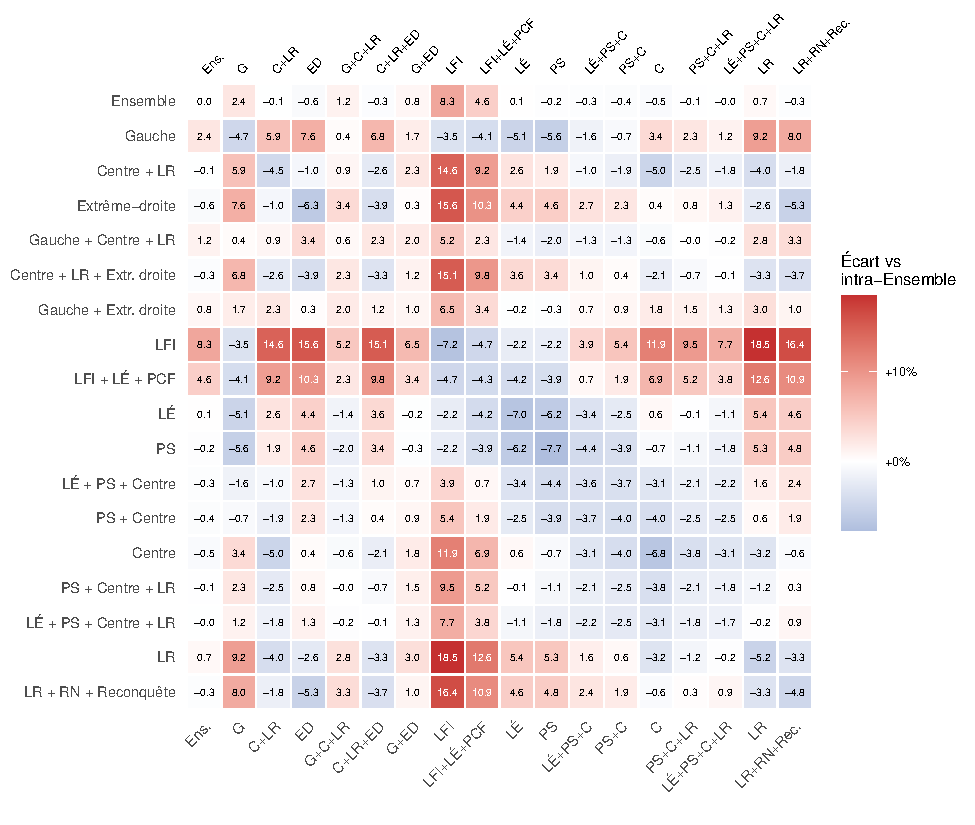
\includegraphics[width=\linewidth]{../figures/distance_matrix_pairwise.pdf}
  \caption{Distances par paires entre groupes électoraux (basées sur les préférences budgétaires)}
  \label{fig:distance_matrix_pairwise}
\end{figure}

Cette matrice confirme que trois blocs font sens~: (1) EELV et PS sont plus proches de LFI que du centre~; (2) le centre est plus proche de LR que de PS ou EELV~; (3) LR est plus proche du centre que de l'extrême droite. La structuration ternaire gauche/centre/droite qui domine le débat politique se retrouve donc dans les préférences budgétaires déclarées.

%%%%%%%%%%%%%%%%%%%%%%%%%%%%%%%%%%%%%%%%%%%%%%%%%%%%%%%%%%%%%
\section{Typologies de répondants et de mesures}
\label{sec:clusters}
%%%%%%%%%%%%%%%%%%%%%%%%%%%%%%%%%%%%%%%%%%%%%%%%%%%%%%%%%%%%%

\subsection{Clustering des répondants}

Un clustering $k$-means appliqué à la matrice binaire de soutien identifie trois profils de répondants~:

\begin{enumerate}
  \item \textbf{Frugaux} (20\,\% des répondants)~: soutien fort aux mesures de rationalisation des dépenses publiques~; opposition aux hausses d'impôts sur tous les ménages~; attitude ambivalente sur les mesures anti-immigration.

  \item \textbf{Nationalistes} (49\,\%)~: profil dominant. Fort soutien aux mesures anti-immigration (retrait des aides aux étrangers, suppression de l'AME) combiné à un soutien modéré aux hausses fiscales sur le patrimoine. Ce profil hybride ne correspond à aucune offre partisane existante.

  \item \textbf{Progressistes} (31\,\%)~: fort soutien aux impôts sur la fortune (ISF, droits de succession), très faible soutien aux mesures anti-immigration. Électorat de gauche surreprésenté.
\end{enumerate}

La cohérence entre ces clusters de répondants et le vote déclaré est notable~: les progressistes concentrent les électeurs de gauche, les nationalistes regroupent une partie de l'extrême droite et des non-votants, les frugaux attirent davantage le centre-droit.

\subsection{Clustering des mesures}

Un clustering analogue appliqué aux mesures (selon leur profil de soutien par groupe d'électeurs) identifie trois familles~:

\begin{enumerate}
  \item \textbf{Mesures de droite} (rendement cumulé~: 64~Mds€)~: mesures anti-immigration, gel des aides sociales, report de la retraite. Plébiscitées par les clusters nationalistes et frugaux, rejetées par les progressistes.

  \item \textbf{Mesures impopulaires} (121~Mds€)~: hausses de TVA, de CSG, réduction des remboursements de soins. Rejetées par l'ensemble des clusters, quel que soit le vote.

  \item \textbf{Mesures de gauche} (39~Mds€)~: ISF, droits de succession, taxes sur les revenus du capital, impôt sur les hauts revenus. Soutenues par les progressistes, tolérées par les nationalistes, rejetées par les frugaux.
\end{enumerate}

La figure~\ref{fig:budget_correlations} présente les corrélations entre mesures. On observe notamment~: une forte corrélation entre les mesures anti-immigration (AME et retrait des aides aux étrangers, $r = 0{,}72$), une corrélation positive entre les mesures taxant le patrimoine, et une corrélation négative entre les mesures de réduction de l'État providence et celles taxant les riches — illustrant la fracture entre les deux familles de soutien majoritaire identifiées en section~\ref{sec:paquets}.

\begin{figure}[htbp]
  \centering
  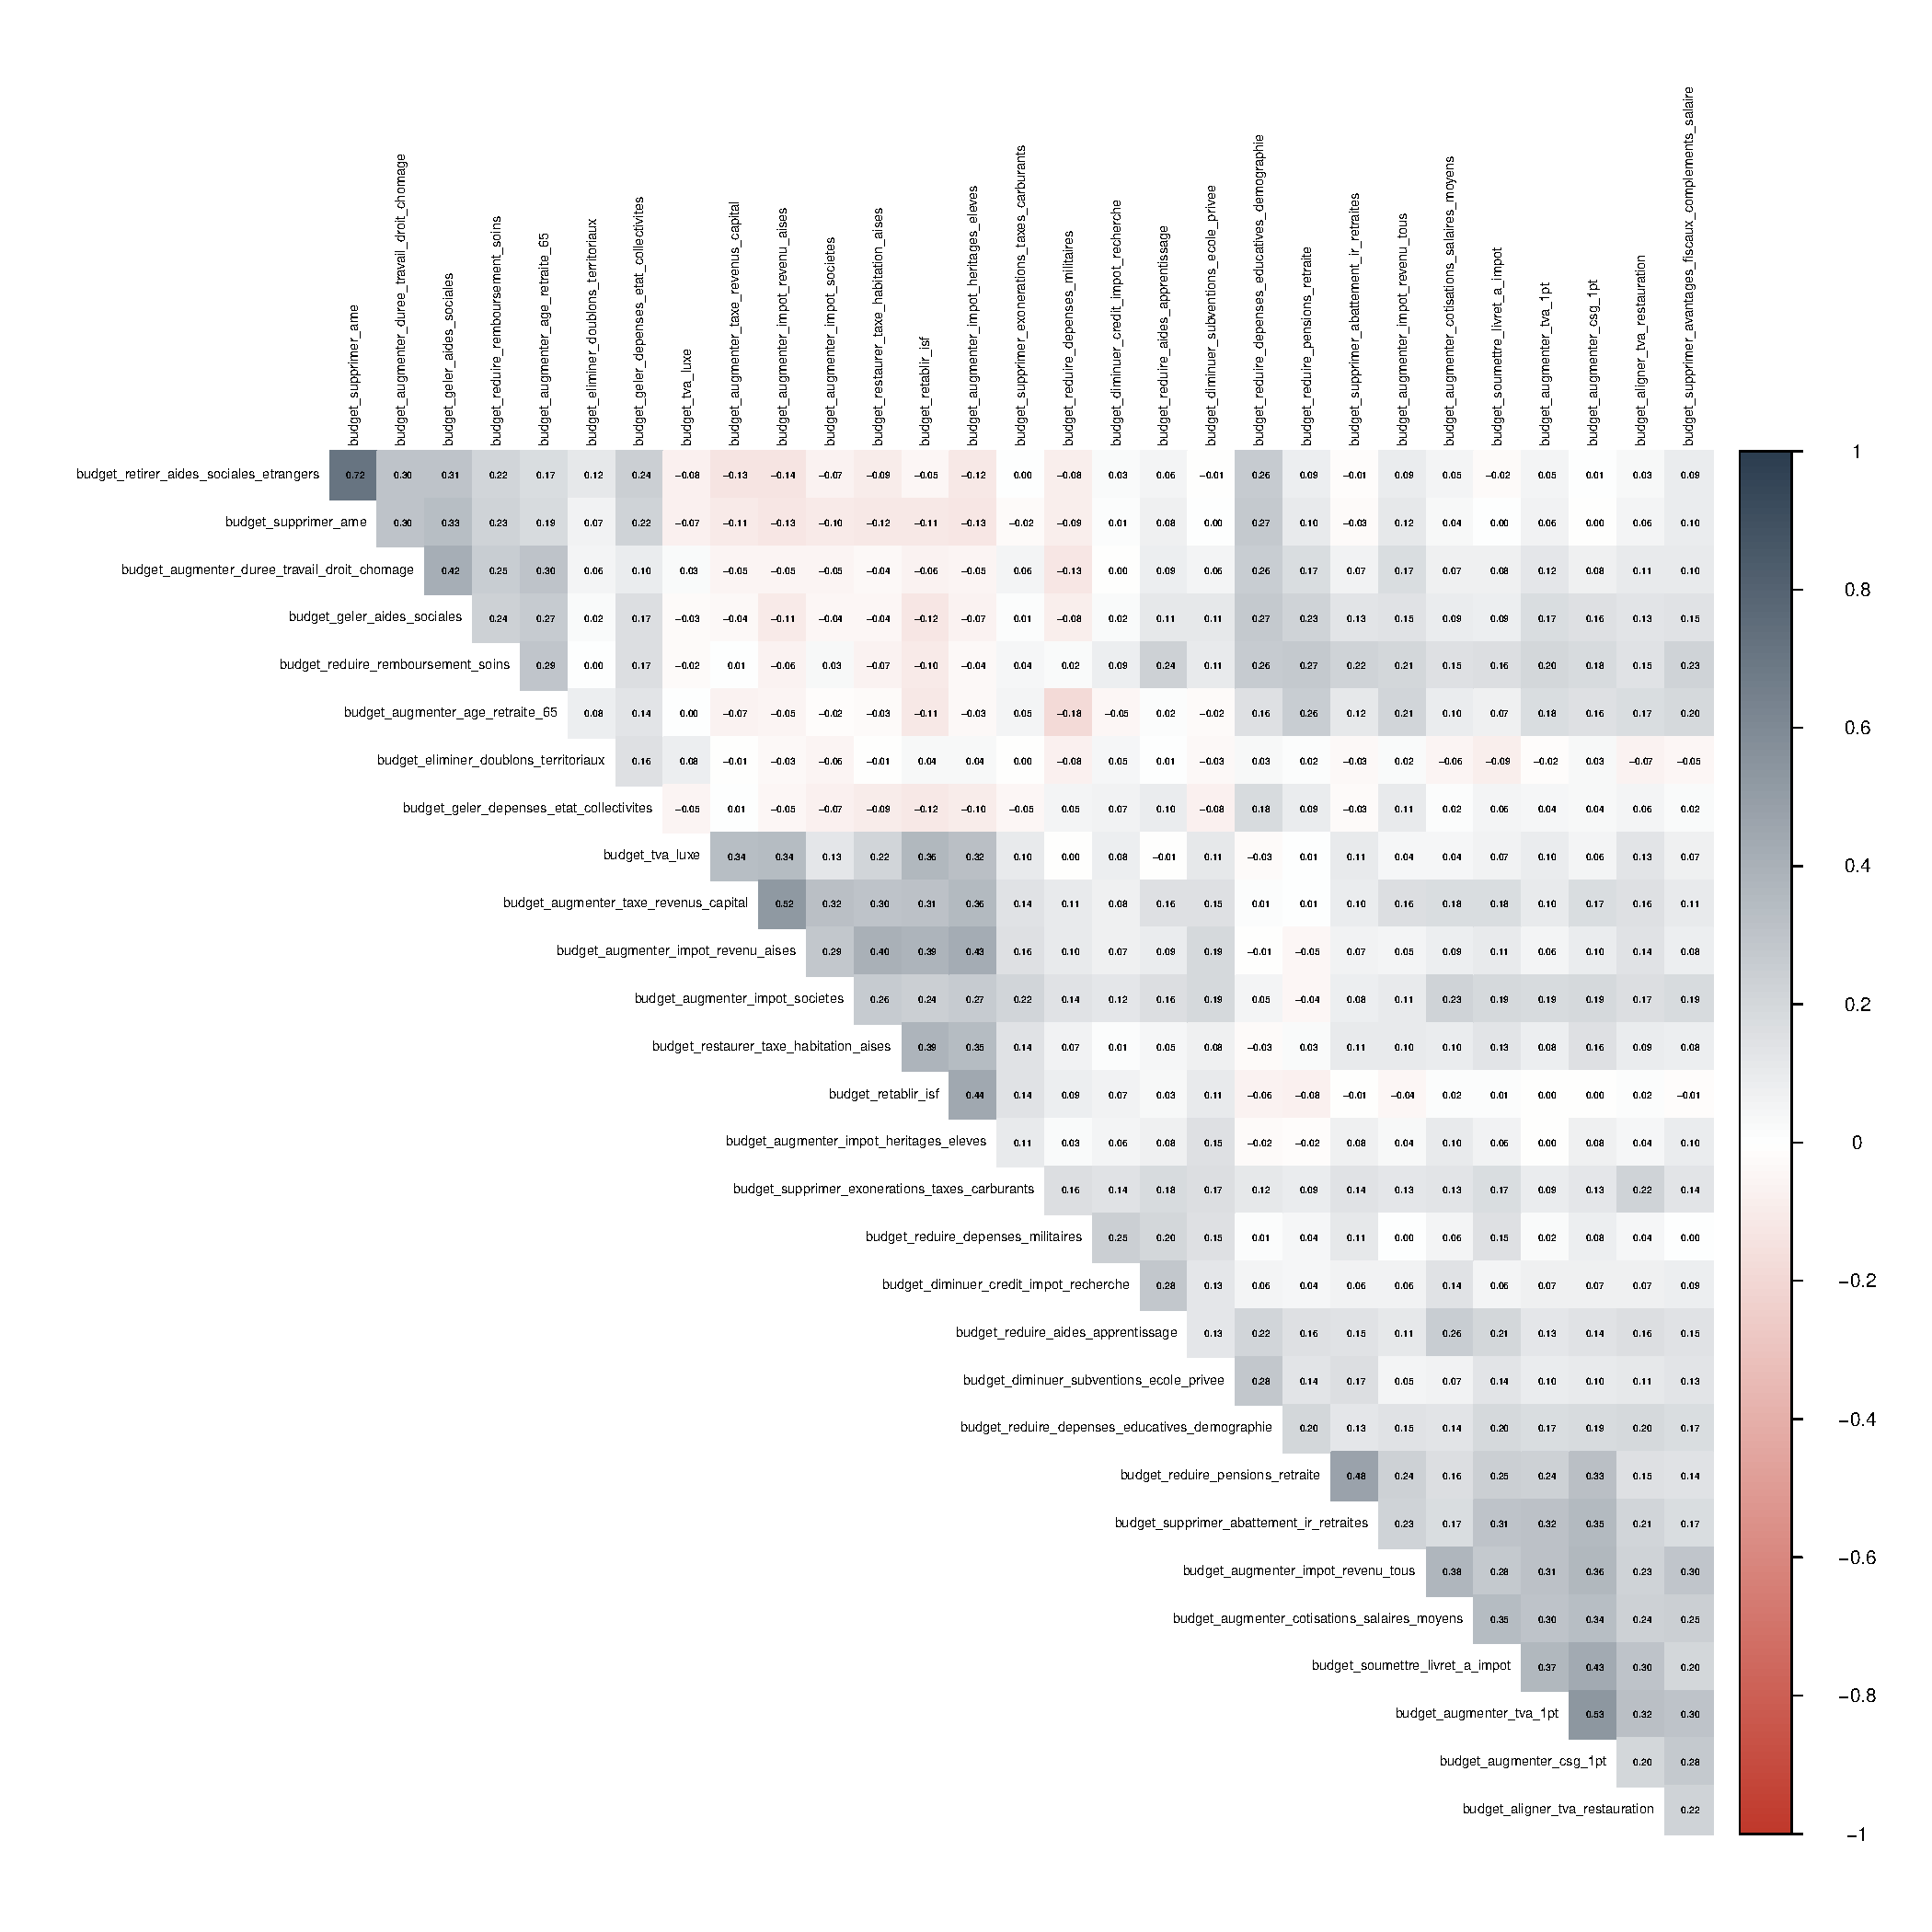
\includegraphics[width=0.85\linewidth]{../figures/budget_correlations.pdf}
  \caption{Matrice de corrélations entre mesures budgétaires}
  \label{fig:budget_correlations}
\end{figure}

%%%%%%%%%%%%%%%%%%%%%%%%%%%%%%%%%%%%%%%%%%%%%%%%%%%%%%%%%%%%%
\section{Comparaison avec Les Progressistes}
\label{sec:progressistes}
%%%%%%%%%%%%%%%%%%%%%%%%%%%%%%%%%%%%%%%%%%%%%%%%%%%%%%%%%%%%%

La plateforme Les Progressistes a organisé fin 2025 une conférence de consensus en ligne~\citep{Progressistes2025}. Les participants à cet exercice ont des préférences budgétaires proches de celles des Écologistes (EELV)~: contrairement aux électeurs de centre-droit, ils sont moins favorables aux mesures de retrait des aides aux étrangers et aux baisses d'impôts sur les entreprises, et davantage orientés vers les mesures écologiques. Par rapport à l'ensemble de l'électorat, les participants aux Progressistes sont moins favorables aux mesures anti-immigration, plus favorables aux taxes sur les riches, et davantage soucieux de la transition écologique.

Ce résultat est cohérent avec le profil sociologique des participants aux exercices de démocratie délibérative en ligne~: ils sont en général plus diplômés, plus à gauche et plus engagés politiquement que l'électeur médian. Il illustre le risque de biais de sélection dans ce type d'exercice, et plaide pour des études d'opinion représentatives comme complément indispensable.

%%%%%%%%%%%%%%%%%%%%%%%%%%%%%%%%%%%%%%%%%%%%%%%%%%%%%%%%%%%%%
\section{Conclusion}
\label{sec:conclusion}
%%%%%%%%%%%%%%%%%%%%%%%%%%%%%%%%%%%%%%%%%%%%%%%%%%%%%%%%%%%%%

Cette enquête apporte plusieurs enseignements.

\textbf{Premièrement}, les Français sont favorables à certaines mesures de consolidation budgétaire, notamment l'élimination des doublons administratifs, les impôts sur le patrimoine (ISF, TVA luxe, droits de succession) et les mesures migratoires. En revanche, ils rejettent les hausses d'impôts touchant l'ensemble de la population (TVA, CSG) et le report de la retraite.

\textbf{Deuxièmement}, la question \texttt{effect\_program} révèle qu'un candidat valorisant à la fois la réduction des dépenses de fonctionnement et l'amélioration des services publics maximise son attractivité — deux objectifs dont la conciliation est difficile. Le retour du déficit sous les 3\,\% du PIB est modérément valorisant.

\textbf{Troisièmement}, les résultats sur les paquets majoritaires illustrent la difficulté à gouverner~: le plus grand paquet de mesures soutenu conjointement par une majorité atteint 68~milliards d'euros, loin des 112~milliards nécessaires. Les paquets majoritaires sont fracturés politiquement (familles anti-immigration et impôts sur la fortune incompatibles avec la définition stricte~; partiellement réconciliables avec la définition élargie).

\textbf{Quatrièmement}, la structuration de l'électorat en trois blocs (gauche, centre, droite nationaliste) se retrouve dans les préférences budgétaires. L'écart entre les préférences individuelles et celles du parti pour lequel chacun a voté est important~: la majorité de la variance est intragroupe, ce qui contribue à l'insatisfaction généralisée envers l'offre politique.

\textbf{Limites.} L'enquête mesure des préférences déclarées sur des mesures individuelles présentées sans contexte de contrainte budgétaire globale~; les citoyens n'ont pas à arbitrer entre mesures ni à équilibrer un budget. Les taux de soutien pourraient différer si les mesures étaient présentées dans un cadre de choix contraint. Par ailleurs, certaines mesures populaires soulèvent des questions constitutionnelles (retrait des aides aux étrangers, restauration de la taxe d'habitation) ou supposent d'autres réformes impopulaires (les économies sur les doublons territoriaux impliquent des suppressions de postes).

\bigskip

\bibliographystyle{plainnaturl_clean}
\bibliography{budget}

%%%%%%%%%%%%%%%%%%%%%%%%%%%%%%%%%%%%%%%%%%%%%%%%%%%%%%%%%%%%%
% \appendix

\end{document}
